\documentclass[UTF8]{ctexart}
\usepackage{graphicx} % Required for inserting images
\usepackage{amsmath}
\usepackage{listing}

\pagestyle{plain}	%取消页眉
\usepackage{fontspec}
\usepackage{geometry}
\usepackage{float}   %H选项打开
\addtocounter{MaxMatrixCols}{10} %矩阵列数大于10
\title{RL Homework 2}
\author{20241202239}
\date{September 2024}
\begin{document}
	
	\maketitle
	\paragraph{Language:} Python
	
	\paragraph{Problem setup}
	\textbf{Environment:} 4*4 grid world.
	\textbf{Reword:} is $r_{boundary} = r_{forbidden}=-1$, and $r_{target}=1$. 
	\textbf{Discount rate:} is $\gamma =0.9$
	\paragraph{Two policies}
	
	Two policies is used,the determined policy is an array [1,1,1,0,1,2,4,0,2,4,4,3,2,3,4,2], where index is related to state, value is related to action.
	We have 
	\begin{equation}
		r_\pi= \begin{pmatrix}
			0\\
			0\\
			0\\
			0\\
			0\\
			0\\
			0\\
			0\\
			1\\
			0\\
			0\\
			0\\
			0
		\end{pmatrix}
	\end{equation}
	and 
	\begin{equation}
		P_\pi= 
		\begin{bmatrix}
			0 & 1 & 0 & 0 & 0 & 0 & 0 & 0 & 0 & 0 & 0 & 0 & 0 \\
			0 & 0 & 1 & 0 & 0 & 0 & 0 & 0 & 0 & 0 & 0 & 0 & 0 \\
			0 & 0 & 0 & 1 & 0 & 0 & 0 & 0 & 0 & 0 & 0 & 0 & 0 \\
			0 & 0 & 0 & 0 & 0 & 0 & 1 & 0 & 0 & 0 & 0 & 0 & 0 \\
			0 & 0 & 0 & 0 & 0 & 1 & 0 & 0 & 0 & 0 & 0 & 0 & 0 \\
			0 & 1 & 0 & 0 & 0 & 0 & 0 & 0 & 0 & 0 & 0 & 0 & 0\\
			0 & 0 & 0 & 0 & 0 & 0 & 0 & 0 & 0 & 1 & 0 & 0 & 0\\
			0 & 0 & 0 & 0 & 1 & 0 & 0 & 0 & 0 & 0 & 0 & 0 & 0 \\
			0 & 0 & 0 & 0 & 0 & 0 & 0 & 0 & 1 & 0 & 0 & 0 & 0 \\
			0 & 0 & 0 & 0 & 0 & 0 & 0 & 0 & 1 & 0 & 0 & 0 & 0 \\
			0 & 0 & 0 & 0 & 0 & 0 & 0 & 1 & 0 & 0 & 0 & 0 & 0 \\
			0 & 0 & 0 & 0 & 0 & 0 & 0 & 0 & 0 & 0 & 1 & 0 & 0\\
			0 & 0 & 0 & 0 & 0 & 0 & 0 & 0 & 0 & 1 & 0 & 0 & 0 \\
		\end{bmatrix}
	\end{equation}
	The stochastic policy is show as follow table, rows related to state, columns related to action,values is probability to take this action. The probability of stay is set to zero, and each boundary action is also set to zero to fasten the policy.
	We have
	\begin{equation}
		r_\pi= \begin{pmatrix}
			0\\
			0\\
			-0.33\\
			0\\
			0\\
			-0.5\\
			-0.33\\
			-0.33\\
			-0.75\\
			-0.33\\
			0\\
			-0.67\\
			-0.33
		\end{pmatrix}
	\end{equation}
	and
	\begin{equation}
		P_\pi= \begin{bmatrix}
			0 & 0.5 & 0 & 0 & 0.5 & 0 & 0 & 0 & 0 & 0 & 0 & 0 & 0 \\
			0.33 & 0 & 0.33 & 0 & 0 & 0.33 & 0 & 0 & 0 & 0 & 0 & 0 & 0 \\
			0 & 0.33 & 0.33 & 0.33 & 0 & 0 & 0 & 0 & 0 & 0 & 0 & 0 & 0 \\
			0 & 0 & 0.5 & 0 & 0 & 0 & 0.5 & 0 & 0 & 0 & 0 & 0 & 0 \\
			0.33 & 0 & 0 & 0 & 0 & 0.33 & 0 & 0.33 & 0 & 0 & 0 & 0 & 0 \\
			0 & 0.25 & 0 & 0 & 0.25 & 0.5 & 0 & 0 & 0 & 0 & 0 & 0 & 0\\
			0 & 0 & 0 & 0.33 & 0 & 0 & 0.33 & 0 & 0 & 0.33 & 0 & 0 & 0\\
			0 & 0 & 0 & 0 & 0.33 & 0 & 0 & 0.33 & 0 & 0 & 0.33 & 0 & 0 \\
			0 & 0 & 0 & 0 & 0 & 0 & 0 & 0 & 0.75 & 0.25 & 0 & 0 & 0 \\
			0 & 0 & 0 & 0 & 0 & 0 & 0.33 & 0 & 0.33 & 0 & 0 & 0 & 0.33 \\
			0 & 0 & 0 & 0 & 0 & 0 & 0 & 0.5 & 0 & 0 & 0.5 & 0 & 0 \\
			0 & 0 & 0 & 0 & 0 & 0 & 0 & 0 & 0 & 0 & 0.33 & 0.67 & 0\\
			0 & 0 & 0 & 0 & 0 & 0 & 0 & 0 & 0 & 0.5 & 0 & 0 & 0.5
		\end{bmatrix}
	\end{equation}
%	\begin{table}[H]
%		\centering
%		\begin{tabular}{|c|c|c|c|c|}
%			\hline
%			0.5   & 0.5   & 0     & 0     & 0 \\ \hline
%			0.333 & 0.333 & 0     & 0.333 & 0 \\ \hline
%			0.333 & 0.333 & 0     & 0.333 & 0 \\ \hline
%			0.5   & 0     & 0     & 0.5   & 0 \\ \hline
%			0.333 & 0.333 & 0.333 & 0     & 0 \\ \hline
%			0.25  & 0.25  & 0.25  & 0.25  & 0 \\ \hline
%			0.25  & 0.25  & 0.25  & 0.25  & 0 \\ \hline
%			0.333 & 0     & 0.333 & 0.333 & 0 \\ \hline
%			0.333 & 0.333 & 0.333 & 0     & 0 \\ \hline
%			0.25  & 0.25  & 0.25  & 0.25  & 0 \\ \hline
%			0.25  & 0.25  & 0.25  & 0.25  & 0 \\ \hline
%			0.333 & 0.333 & 0.333 &   0   & 0 \\ \hline
%			0     & 0.5   & 0.5   & 0.    & 0 \\ \hline
%			0     & 0.333 & 0.333 & 0.333 & 0 \\ \hline
%			0     & 0.333 & 0.333 & 0.333 & 0 \\ \hline
%			0     & 0.    & 0.5   & 0.5   & 0 \\ \hline
%		\end{tabular}
%	\end{table}

	Here plot the tow policies.
	\begin{figure}[H]
				\centering
				\begin{minipage}[t]{0.48\textwidth}
						\centering
						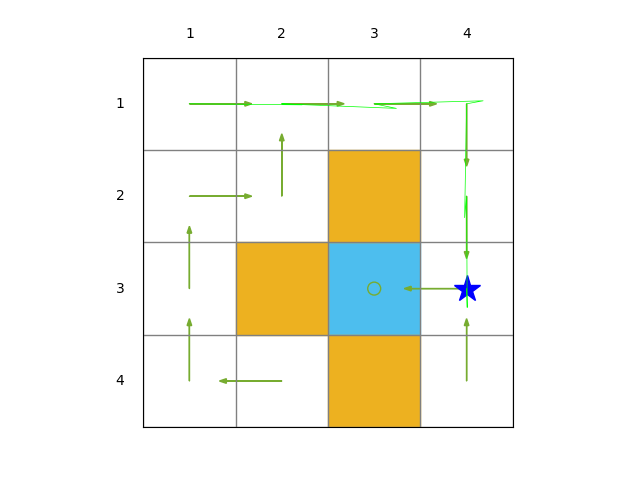
\includegraphics[width=6cm,height=6cm]{fig/policy1}
						\caption{Policy 1}
					\end{minipage}
				\begin{minipage}[t]{0.48\textwidth}
						\centering
						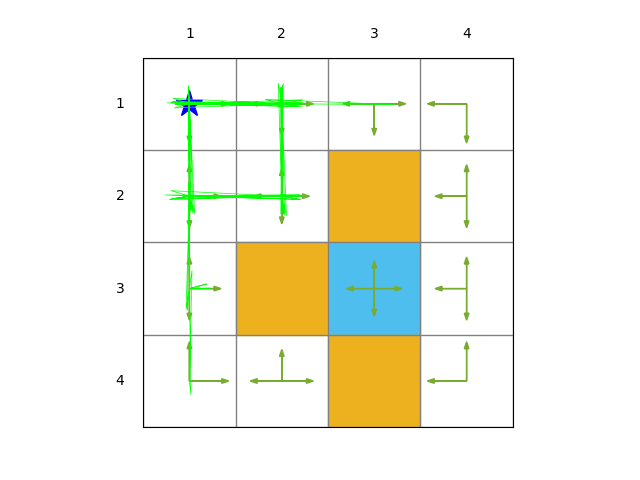
\includegraphics[width=6cm,height=6cm]{fig/policy2}
						\caption{Policy 2}
					\end{minipage}
	\end{figure}
	
	\subparagraph{closed-form algorithm} $v_\pi = (I - \gamma P_\pi)^{-1}r_\pi$ is directly transformed from Bellman equation $v_\pi = r_\pi+\gamma P_\pi v_\pi$, it's useful for theoretical analysis, but not applicable for computer calculate because it involves matrix inversion operation. Here plots state value calculated from closed-form algorithm.
	\begin{figure}[H]
		\centering
		\begin{minipage}[t]{0.48\textwidth}
			\centering
			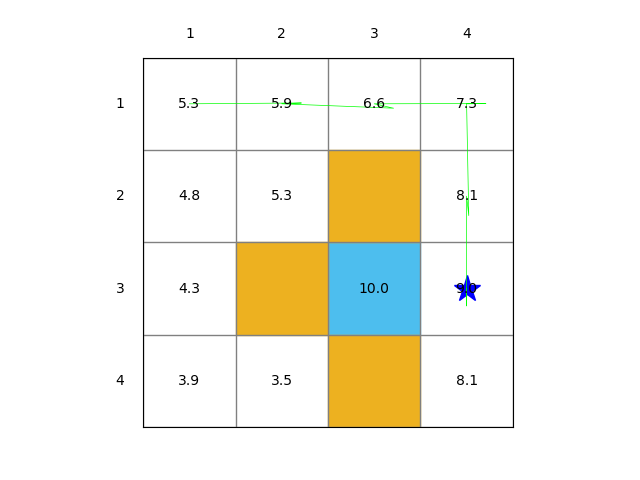
\includegraphics[width=6cm,height=6cm]{fig/policy1_closed}
			\caption{Policy 1}
		\end{minipage}
		\begin{minipage}[t]{0.48\textwidth}
			\centering
			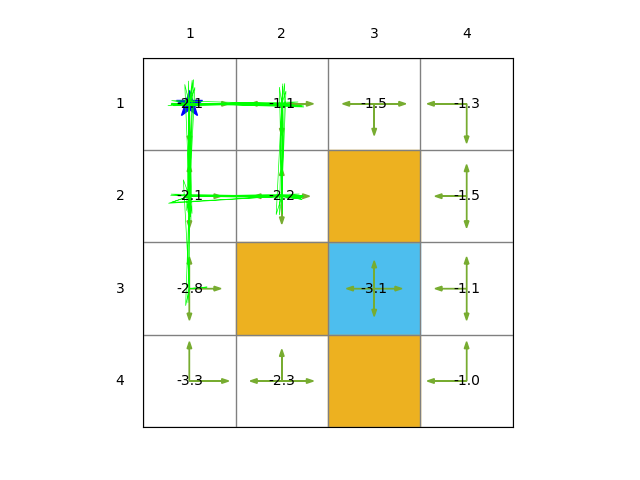
\includegraphics[width=6cm,height=6cm]{fig/policy2_closed}
			\caption{Policy 2}
		\end{minipage}
	\end{figure}
	\subparagraph{iterative algorithm} $v_{k+1} = r_\pi + \gamma P_\pi v_{k}$ is using fix point iterative solution to find $v_\pi$, it is easier to calculate. Here plots state value calculated from iterative algorithm, $v_0$ uses all one array and 100 iteration is applied.
	\begin{figure}[H]
		\centering
		\begin{minipage}[t]{0.48\textwidth}
			\centering
			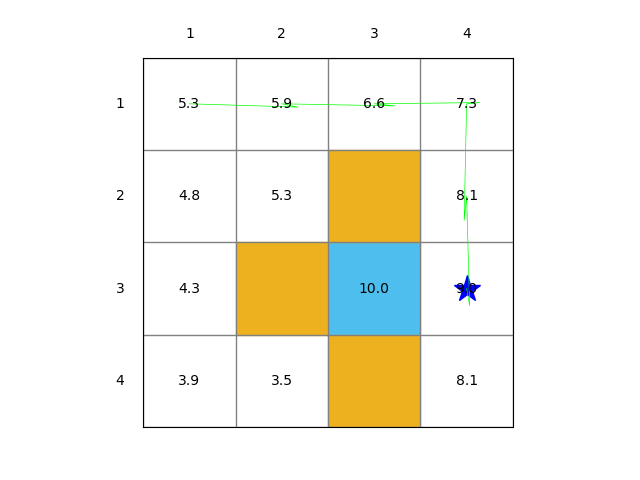
\includegraphics[width=6cm,height=6cm]{fig/policy1_interative}
			\caption{Policy 1}
		\end{minipage}
		\begin{minipage}[t]{0.48\textwidth}
			\centering
			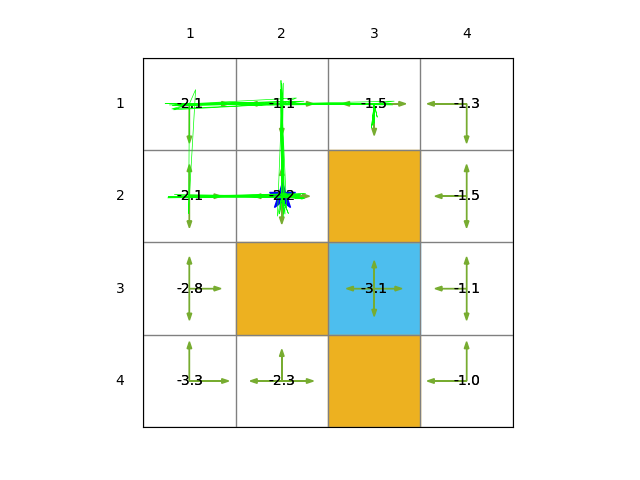
\includegraphics[width=6cm,height=6cm]{fig/policy2_interative}
			\caption{Policy 2}
		\end{minipage}
	\end{figure}
	\paragraph{Observation} For deterministic policy 1, state value decrease with the distance goes far. For policy 2, most state values decrease with the distance goes far, but the states near the forbidden state have lower state value. Also compare policy 1 to policy 2, policy 1 generally have higher state value.

\end{document}